\documentclass[a4paper,11pt]{article}
\usepackage[T1]{fontenc}
\usepackage[utf8]{inputenc}
\usepackage{lmodern}
\usepackage{graphicx}
\usepackage[top=2cm, bottom=2cm, left=2cm, right=2cm]{geometry}
\usepackage{subcaption}
\usepackage{hyperref}

\title{INFO-F-404~: Real-Time Operating Systems\\Project 2~: Bitonic}
\author{Rémy Detobel, Stanislas Gueniffey and Denis Hoornaert}

\begin{document}

\maketitle

\section{Implementation choices}

  Typically, there are two main types of process~: the \textit{master node} and the \textit{compute node}. Each node has its own purpose(s) and interact with the other processes using \textit{MPI}.\\
  
  \noindent There is only one \textit{master node} per program instance. Its objective is to oversee and deal \textit{merge tasks} to its \textit{compute nodes}. Typically, the \textit{master node} will, when a non-bitonic list is given, execute multiple successive merge call so that the list will be \textit{bitonic} before performing the sort itself. Afterwards, the sorting  ---which consists of a merge of the whole list--- is performed.\\
  
  \noindent The \textit{compute nodes} have for only mission to compare two values and to determine to which other \textit{compute node} they have to send the outcome of the comparison. The mechanism is as follow~:\\
  Initially, each \textit{compute node} receives two values from the master node. Then a first comparison is done. After having complete the comparison, the outcome is send to another \textit{compute node} as mentioned above, a new value (coming from another \textit{compute node} having performed the same mechanism) is received and another comparison is performed.\\
  The number of comparisons and the determination of both the sending \textit{compute node} and the receiving \textit{compute node} are obtained at the runtime. The former is obtained by applying the $\log_{2}$ of the list size whereas the latter are obtained using the following formula~:
  \[dest = (id~xor~(1 << depth)) + 1\]
  Where~:
  \begin{itemize}
    \item $id$ is the process id (or rank) of the current process
    \item $depth$ is the number of comparisons that the compute node still has to perform
    \item $dest$ is the process id of the destination
  \end{itemize}

\section{Project utilisation and configuration}

  As mentioned in the assignment statements, the source code can either be used with a \textit{bitonic} list as input or with an unsorted list.\\
  In the case of a \textit{bitonic} list input, the user is invited to set the macro \verb|SORT_FIRST| (\verb|main.cpp| line 8) to \textit{false}. Doing so, will make the program to sort the hardcoded list written line 74. If the user wants to test the project with a fully random list, he only has to set the macro \verb|RANDOM_LIST| to \textit{true}.\\
  Notice that the list generation does not ensure the generation of a \textit{bitonic} list. Hence, it is required to set the macro \verb|SORT_FIRST| to \textit{true}.\\
  Once that the manipulation have been done, the user is invited to compile the project using the provided Makefile.

\section{Inter-processes communications}

  The implemented inter-processes communication protocol (\ref{fig:sato_comm}) differs a bit from the one suggested in the reference (\ref{fig:impl_comm}). In fact, in order to ease the implementation of the \textit{parallel bitonic sorting algorithm}, it has been decided that after each merge the \textit{compute nodes} have to send their results to the master node instead of dealing themselves with the communication. Consequently, parallelism is not exploited as far as possible and this has an impact on the expected performances.
  \begin{figure}[h!]
    \centering
    \begin{subfigure}[b]{0.4\textwidth}
        \centering
        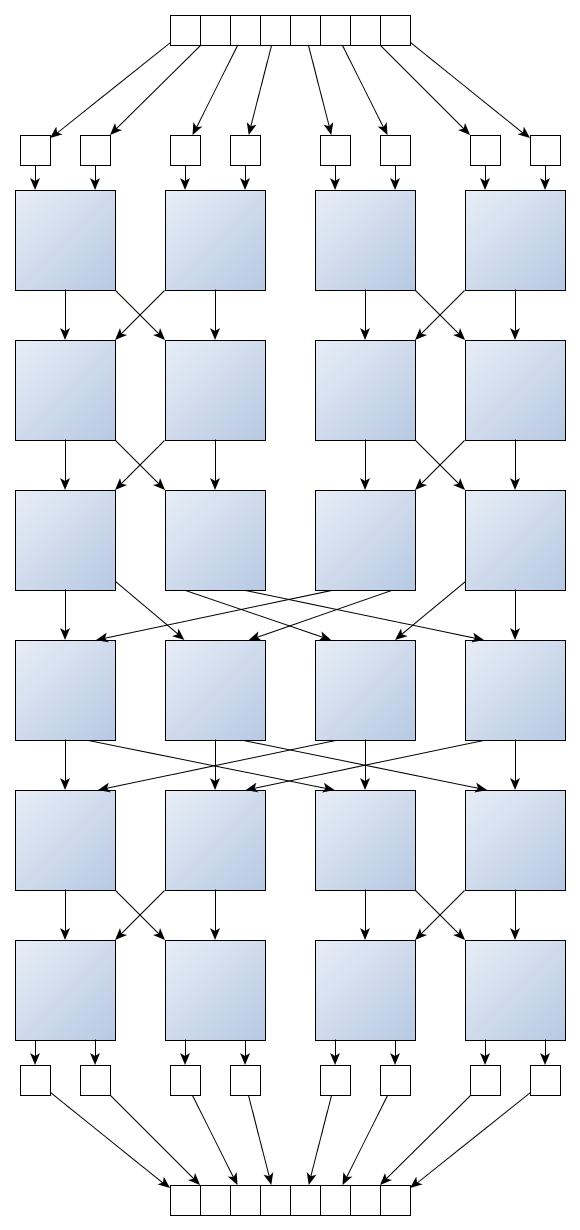
\includegraphics[scale=0.15]{img/bitonic_sort_8_sota.png}
        \caption{State of the art commnucations}
        \label{fig:sato_comm}
    \end{subfigure}
    ~
    \begin{subfigure}[b]{0.4\textwidth}
        \centering
        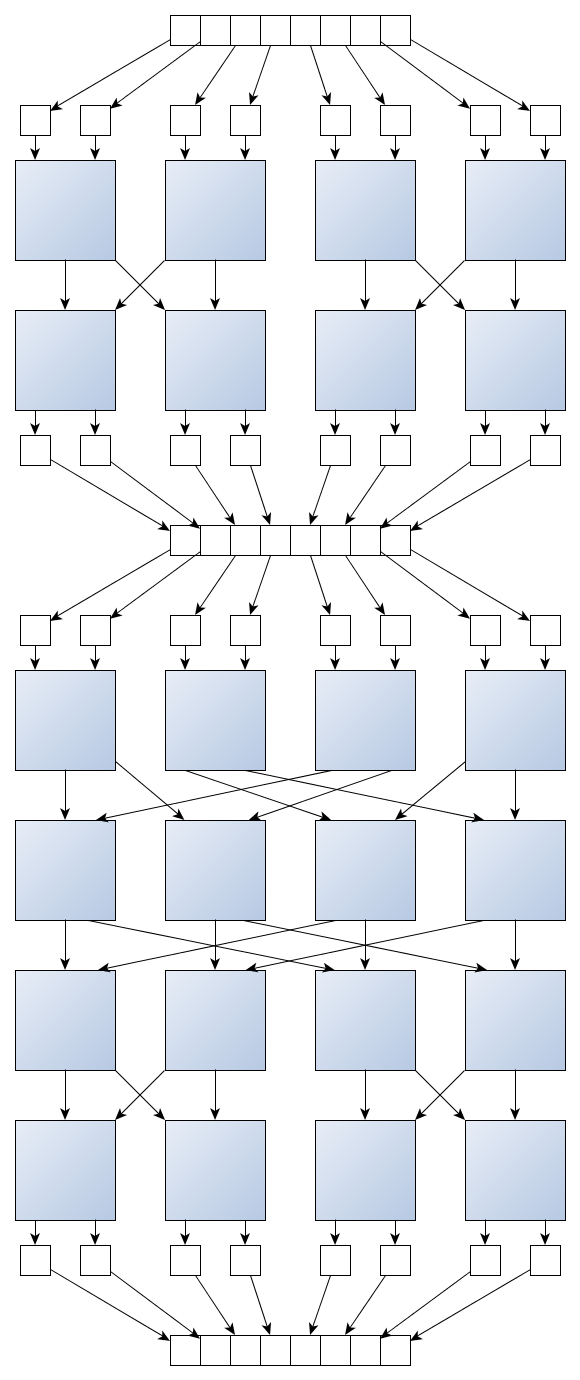
\includegraphics[scale=0.15]{img/bitonic_sort_8.png}
        \caption{Project communications}
        \label{fig:impl_comm}
    \end{subfigure}
    \caption{}
    \label{}
  \end{figure}

\section{Limitations and performances}

\end{document}
